\documentclass[../main.tex]{subfiles}
\graphicspath{{\subfix{../../images/}}}
\begin{document}

\chapter{Experimental Methods}\label{chap:methods}

\bigskip
\begin{quote}
    \emph{We have some idea as to the intricate design of the puppet and the puppet strings, but we lack insight into the mind of the puppeteer\cite{bizziHardScientificQuest2015}.}\\
    \raggedleft{--- Emilio Bizzi \& Robert Ajemian, 2015}
\end{quote}

\cleardoublepage%


\section{Methodological Aims}\label{methods_aims}

\begin{itemize}
  \item Our goal is to explore EMG as a paradigm, particularly with a high degree of redundancy. Most tasks use a few muscles, we want to capture as much of the activity driving the hand as we can using surface EMG
  \item We're interested in the hand because, we argue (with others, mostly anthropologists), that along with language the hand is the most evolutionarily advanced \textit{thing} in the known universe! How we control it \textit{flexibly} is a huge open question, something we have yet to achieve \textit{in silico}
  \item We choose EMG because it is the ``raw'' signal directly from the brain, circumventing constraints and idiosyncrasies of joint kinematics... (this needs more thought, what are these idiosyncrasies?)
  \item We want to develop a task with:
  \begin{itemize}
    \item continuous action space--- not a discrete choice
    \item redundancy--- more input variables (e.g. muscles) than output (task-relevant) variables, and control over the redundant mapping between inputs and outputs
    \item a task that looks more like a new skill, rather than adaptation of a known movement to a contingency (though this is blurry! ``Skill'' is not well defined. (Should we try to define it?))
    \item ``Slow'' learning--- we want to track subjects' progress over many trials. If they learn too quickly, we may miss the subtleties of their progress. This requires us to titrate the difficulty of the task to a degree that makes the taska real challenge for subjects but is learnable. How we attempt to achieve this is explained in \Cref{sec:decoder_fitting}
    \item We want the subject to embody, as much as possible, an infant-like state of ignorance within their bodies. They will understand the task intellectually (as its simple to explain the goal) but there is no ``trick'' to the task, it simply requires using your muscles in a new way
  \end{itemize}
  \item The questions our paradigm should allow us to access are:
  \begin{itemize}
    \item Do we learn ``from scratch'' or \textit{de novo}? Or do we reconfigure existing primitives?
    \item Do we uncover to task redundancy and use this to our advantage from the beginning of learning?
    \item 
  \end{itemize}
\end{itemize}

This is a step beyond recording hand kinematics as electromyography provides a physiological output of the nervous system. Surface electromyography recordings taken from the forearms controlling subjects' dominant hands allows us to track the sequential selection of muscle activations during both skill acquisition and subsequent performance of that skill to achieve desired goal. As we are interested in subjects' abilities to acquire new skills, we design tasks that require subjects to use available, but uncommon, motor activations. We then track the selection and execution of these activation during virtual tasks. Preliminary work in this direction is described in \cref{sec:experiment}.

The concept of the experimental setup is shown in \Cref{fig:setup}, where 32 monopolar electrodes are attached to a subject's forearm to record muscle activity. The arm and hand are kinematically constrained in a custom fixture and motor activity is recorded during low-level isometric muscle contractions. The setup circumvents the limb biomechanics by mapping muscle output directly to virtual stimuli shown on a screen. By focusing on low-force, isometric contractions we intend to avoid complications due to artifacts in dynamic, high-force movements.

The concept of redundancy is common: in the human perception of color, we have a 3-dimensional plane of perception red, green, blue, while the space of physical colors is an infinite-dimensional spectrum. Thus, we can perceive some colors (e.g. yellow light vs. green+red light) with different spectra as identical, as they are identical when ``projected'' onto our perceptual plane (this is known as metamerism).


\section{Recording Setup}\label{hardware}

Describe the experimental setup/environment, what is taking place in each session, protocol, software, hardware, how the signal is captured, physical setup

0. enter subject details, arrange filepaths appropriately
   1. make a data folder for each subject, with experimental not
   2. make subject info json (to be picked up by python later)
1. clean and prep arm
   1. soap and water, scrub
2. attach electrodes at a fixed position
   1. measure arm at ulnar styloid
   2. measure arm 5cm from elbow tip
   3. where to place band?
3. set up arm in enclosure, attach ground
4. test recording
   1. **validation: visual inspection of data**
      1. noise
      2. electrode liftoff / seating
      3. in case of issues, adjust sleeve etc. accordingly
5. explain natural movement task
   1. you will be asked to perform a series of movements:
      1. read each movement and demonstrate
      2. try to the best of your ability
      3. don't need to use maximum force, approx 50% of maximum at peak
   2. once the subject is ready, the task (rest + movements) is run 3 times
6. bar calibration task
   1. you will be asked to perform an exploration and isolation task
   2. you will see 64 vertical bars on your screen
   3. your movements cause the bars to change height
   4. the goal of each trial is to maximize the height of the red bar whilst minimizing the height of all other bars
   5. to the best of your ability
7. scripts are run to produce modes and choose decoder
   1. **validation: modes are visually inspected**
   2. if an error is seen, emg is checked, calibration is repeated
   3. if modes look reasonable, continue to task
8. center hold task
   1. you will be asked to move a dot to target locations on the screen using muscles controlling your hand movements. first you must hold the dot in the center of the screen for a required time, after which a trial will begin. each trial you will attempt to move the dot towards the target and hold it there for a desired time. if you are successful, a new trial will begin. if you run out of time, a new trial will begin.
- run task for desired number of trials for a range of targets.
- after each run, briefly interview the subject about discomfort, feeling, strategies, glaring errors (only doing one movement), etc.



\begin{figure}[tph]
\centering
\includegraphics[width=1.0\textwidth]{methods/setup.pdf}
\caption[Experimental setup prototype]{(a) Graphic depicting the closed-loop EMG interface concept in a center-hold, reach-out type task. The multidimensional EMG signal is transformed online through a mapping $F$ from EMG electrode space to a lower dimensional task space, creating an experimentally controllable redundancy problem for the subject. In experiments shown here the task space is two-dimensional, though the EMG interface can be extended to tasks with higher-dimensional inputs. The subject's arm and hand are constrained during the experiment to ensure isometric contractions. (b) First prototype of custom recording hardware consisting of four bands of eight electrodes each, and a spherical hand constraint. Our recordings are 32 channel monopolar recording with reference electrode at the wrist. (c) Example cup-style monopolar recording electrodes, 5mm in diameter. (d) Side view of the recording hardware. Also pictured is the arm restraint frame to ensure isometric contractions. The frame obscures the subject's arm from view and contains adjustable elbow and wrist rests. (d) Recording hardware shown off the arm with wireless amplifier and connection board.}\label{fig:setup}
\end{figure}

As far as we are aware, this setup is novel in combining a high number of channels with an abstract mapping. Learning experiments have used joint angles and a few muscles (typically movements of the wrist or pairs of thumb and intrinsic hand muscles), but none have taken a data-driven approach in constructing a virtual learning environment in the style of cortical BMI\cite{@BergerDifferencesInAdaptationRates2013a;@Dyson2018;@radhakrishnanLearningNovelMyoelectricControlled2008;@Gallego2017}. Our EMG recording setup is custom-built: the ``Sessantaquattro'' EMG amplifier was acquired from OT Bioelettronica, the electronic connector was designed in-house, the electrodes were acquired from Medkit UK, and the recording software was written in a mixture of Bonsai (C\#) and Python. EMG is acquired at 2kHz sample rate with 24-bit precision. A clip of raw data is shown in \Cref{fig:raw_data}.


\begin{figure}[tph]
  \centering
  \begin{minipage}{0.33\textwidth}
    \includegraphics[width=\textwidth]{methods/electrode_assembly.png}
    \subcaption{}
  \end{minipage}%
  \hspace*{5pt}
  \begin{minipage}{0.33\textwidth}
    \includegraphics[width=\textwidth]{methods/electrode_detail.JPG}\\
    \subcaption{}
    \includegraphics[width=\textwidth]{methods/hand_constraint_detail.JPG}
    \subcaption{}
  \end{minipage}%
  \hspace*{5pt}
  \begin{minipage}{0.33\textwidth}
    \includegraphics[width=\textwidth]{methods/hand_constraint_in_box.JPG}\\
    \subcaption{}
    \includegraphics[width=\textwidth]{methods/peter_playing_game.JPG}
    \subcaption{}
  \end{minipage}
  \caption[Experimental setup]{(a)  (b)  (c)  (d)}\label[figure]{final_setup}
\end{figure}

\begin{figure}[tph]
  \centering
  \includegraphics[width=1.0\textwidth]{methods/muscle_map.pdf}
  \caption[Electrode layout with forearm and hand muscles]{}\label{fig:muscle_map}
\end{figure}



\section{Raw Data}

\begin{figure}[tph]
  \centering
  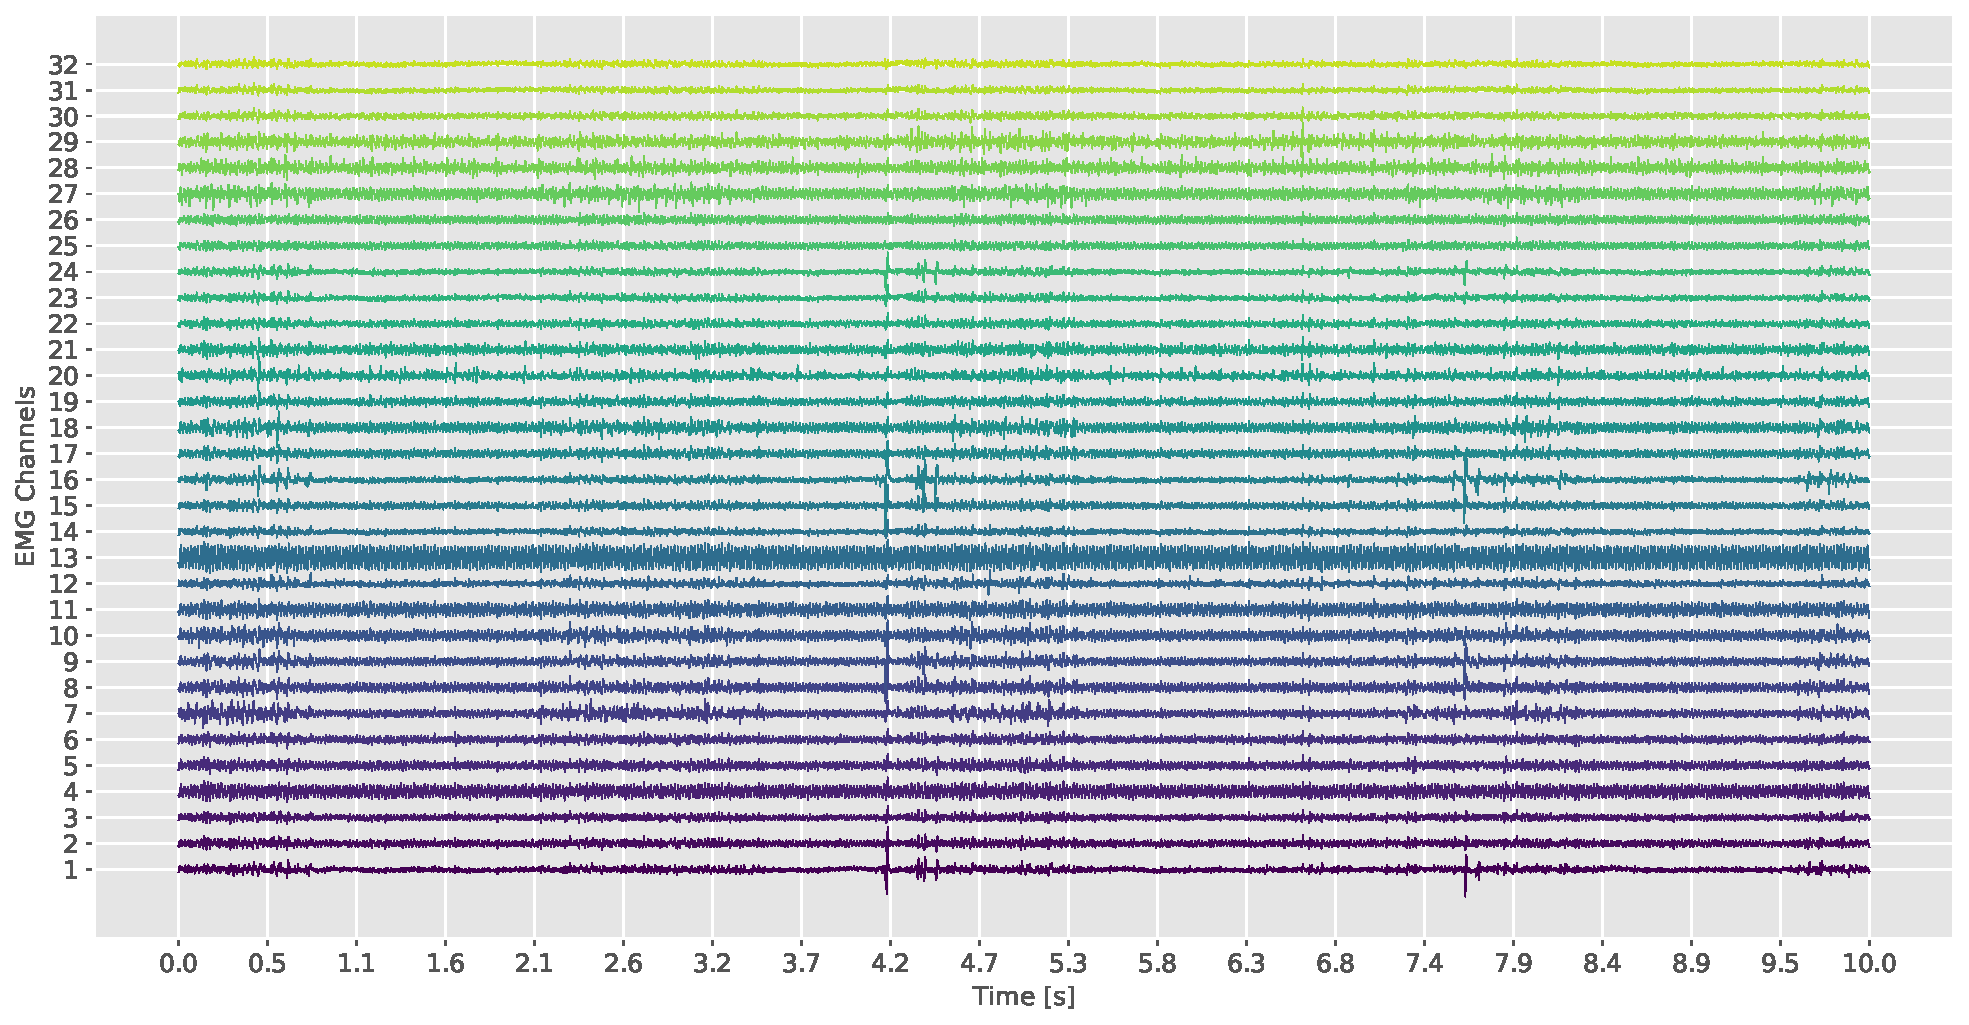
\includegraphics[width=1.0\textwidth]{methods/raw_data.pdf}
  \caption[Example raw EMG data]{Notice: highly correlated across channels, artefacts and noise. \\ 10 seconds of raw 64-channel EMG data taken during a minimal finger flexion trial. Note that some channels include a nontrivial amount of line noise. This noise will be drastically reduced through changes being made in the next recording hardware revision which include shielding, shorter cables, and better cable routing. Note that some channels (e.g. channel 24) show very low noise and putative single motor unit action potentials can be seen on many channels.}\label{fig:raw_data}
\end{figure}


\section[]{Tasks}

\begin{figure}[tph]
  \centering
    \includegraphics[width=1.0\textwidth]{methods/task_structure.pdf}
    \caption[Movement task visual feedback]{}\label{fig:movement_task_screen}
  \end{figure}


\subsection{Natural Movement}

In our first preliminary experiment, a single subject produced flexions and extensions of each finger in the recording setup without any kind of artificial feedback. One trial was collected per finger movement in three blocks per session and one session per day over five days for a total of fifteen trials per finger movement. The purpose of this experiment is to determine the robustness over trials and sessions of EMG features for a simple low-contraction movement, as well as to determine the level of noise and artifacts in the data. Such baseline measurements are important to properly decompose variability due to electrode placement and exogenous noise from behavioral and physiological variability in order to ensure reproducibility of our results. Additionally, this baseline task may prove useful as a benchmark for later tasks in terms of testing analysis and decomposition techniques. A plot of all 32 channels for a single trial after preprocessing is shown in \Cref{fig:preprocessed_data}.

% \begin{figure}[tph]
% \phantomsection\label{fig:preprocessed_data}
% \centering
% 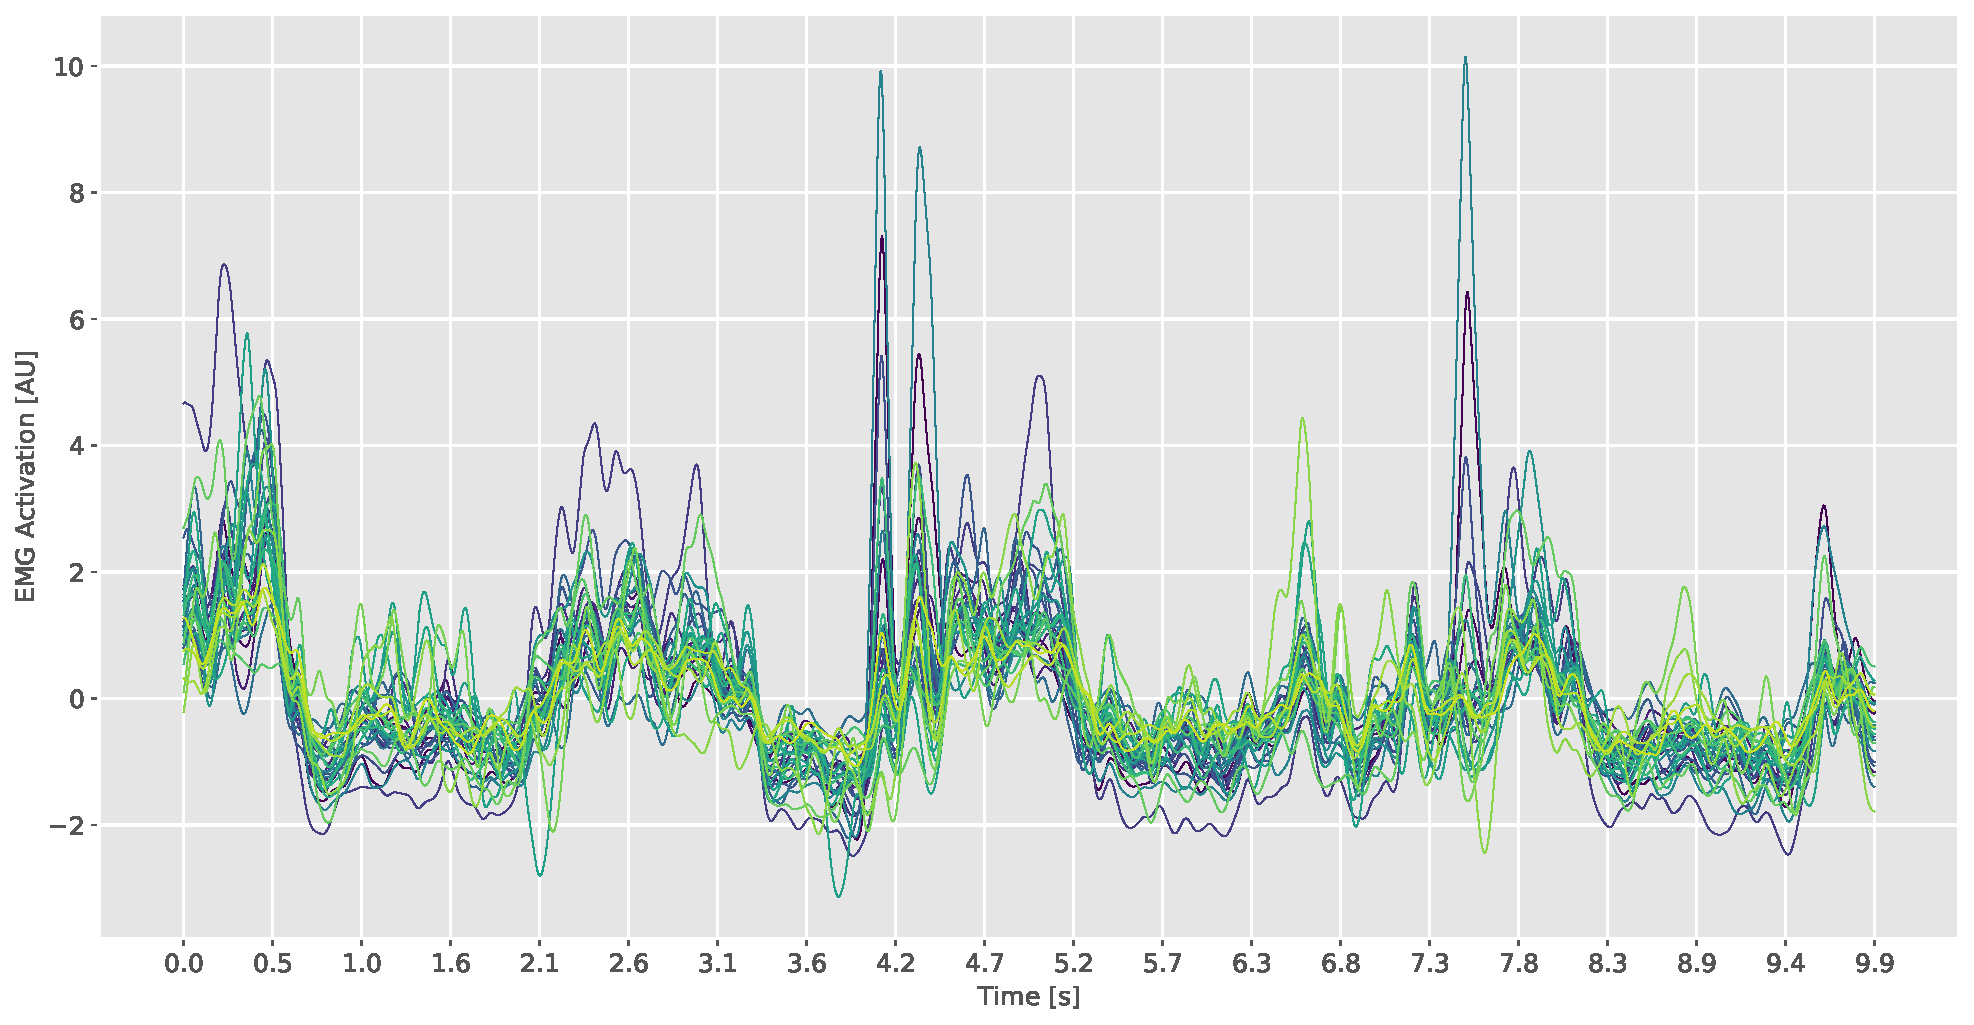
\includegraphics[width=0.2\textwidth]{images/data_analysis/fingers/preprocessed_data.pdf}
% \caption{All channels of data from a single trial after preprocessing.Note the difference in baseline for each channel. Ideally, each channelhas a clear baseline of no activity, as further discussed in the main text.}\label{fig:preprocessed_data}
% \end{figure}



\subsection{Calibration}

Goal: What is the best calibration task to find the boundaries of the available EMG space? 

Does this work?? Can we quantify whether people are actually exploring the space?

To preprocessing the data, simple filtering and rectification were applied, as is commonly done in the literature\cite{@sangerBayesianFilteringMyoelectric2007;@churchlandNeuralPopulationDynamics2012a;@churchlandNeuralVariabilityPremotor2006;@sussillo2015}. As shown in \Cref{fig:preprocessing_steps}, here we apply highpass filtering at 40Hz to remove any low-frequency oscillations and DC offsets, rectification and lowpass filtering at 5Hz to extract what is typically associated with a force readout of the EMG signal in the case that electrodes are positioned over the belly of a single muscle. These filter parameters were chosen by visual comparison across a range of values. While these preprocessing steps are in accordance with the literature and yield a signal with frequencies on a behavioral timescale though, as discussed in \Cref{sec:next_steps}, preprocessing of raw EMG signals is an area worth investigating the development and application of more advanced methods.



\subsubsection{Does the Calibration Task Encourage Exploration?}

Compare to the Movement task! Calibration will show higher variance (maybe look at the determinant of the covariance? across subjects?)

Are people “better” than random EMG at the calibration task? How do we define the “null” hypothesis here, what is comparable random EMG? (E.g. sample from a distribution with the same statistics)

Hypothesis: subjects aren’t moving randomly in this task. They are goal-oriented and are using feedback to solve this search problem.
  
  
 
\subsection{Decoder Fitting}\label{sec:decoder_fitting}

\textbf{How is the decoder derived? Why this way? What does this mean geometrically?}


Electrode data from a single trial of a single session is held in a data matrix $X$ (n\_electrodes, n\_samples), and we wish to find a latent weight matrix $W$ (n\_electrodes, n\_components) which reconstructs $X$ by projecting latent trajectories $H$ (n\_components, n\_samples) into electrode space:

\begin{align*}
X = W\cdot{H}
\end{align*}

$H$ is the activity of the latent processes, and $W$ is there mixing matrix. The columns of $W$ are the principal vectors spanning the latent subspace in electrode space. If we have new samples, we can project these new points onto this subspace:

\begin{align*}
h_{new} = W^T\cdot{w_{new}}
\end{align*}

To justify this decomposition, we have to make some assumptions about the nature of the EMG signal, namely that the signal is linear instantaneous (each EMG sample can be instantly mapped to control space). The other assumption is that the basis $W$ should be orthonormal, that the columns of $W$ are orthogonal with unity norm. This ensures that the left inverse $W^{-1}$ is equal to the transpose $W^T$ such that:

\begin{align*}
X &= W\cdot{H} \\
W^{-1}\cdot{X} &= {H} \\
W^{T}\cdot{X} &= {H}
\end{align*}

See *Muceli 2014* for use of the Moore-Penrose pseudoinverse in place of the transpose when the columns of $W$ do not form an orthonormal basis. This would be the case for NMF. Is there a factorization that produces nonnegative, orthogonal coordinates? Or is the pseudoinverse okay? I will need to test this.

Stated in an information theoretic way, we want to minimize the reconstruction loss $\mathcal{L}$ for our derived encoder-decoder pair ($E$,$D$). We're decoding high dimensional activity into its latent dimensions, and encoding back into the high dimensional space.

\begin{align}
  \min_{E,D}{\mathcal{L}\left[X - EDX\right]}
\end{align}

This way, forget about orthonormality and solve for an encoder and decoder directly. That is, $E\neq{D}$ is perfectly acceptable.

Each row of $D$ might be called a **spatial filter**, a linear combination of electrode activities into a surrogate, hopefully more intuitive space.


$$WH   =  X$$

TxK x Kx64 = Tx64

transformation x components = data

factors x weights = data

inverse:

$$W = XH^{-1}$$
$$W^T = H^{-T}X^T$$

KxT = Kx64 x 64xT
We're not regularizing here, so the cost function for the fit looks like:

$$\min{||X - WH||^{2}_{loss}}$$


The mapping between EMG and task space $M$ can be written as

\begin{align}
M = \begin{bmatrix}\tilde{M} & \tilde{M} & \tilde{M} & \tilde{M}\end{bmatrix}
\end{align}

where $\tilde{M}$ consists of 8 equally spaced directions, one for
each ``column'' of the 4 EMG electrode bands around the subject's arm:

\begin{align}
\tilde{M} =
\begin{bmatrix}
0  & 0.71  & 1   & 0.71   & 0  & -0.71  & -1  & -0.71 \\
1  & 0.71  & 0  & -0.71  & 1   & -0.71   & 0   & 0.71
\end{bmatrix}
\end{align}

A graphic showing the mappings from electrodes to force directions is shown in \Cref{fig:columns}. While there are 8 possible force vectors the subject can modulate by controlling the electrode activity on each of her 8 columns, the EMG mapping is ultimately a projection onto the 2D plane. Since the EMG signal is nonnegative, the subject could technically modulate just four modes of electrode activity, the minimum number needed to span the task space, to reach all 32 targets. This mapping was chosen in order to provide a simple starting point to explore the virtual EMG task. There are no added environmental dynamics, only a redundant readout of force, and the signal is processed online in the same manner as in the offline analyses. This task or a variant we think can serve as a foundation upon which we can build more complex mappings and virtual environments. Task space trajectories from each block are shown in \Cref{fig:trajectories}. The fraction of trials resulting in hold timeouts, reach timeouts, and target hits are shown over blocks in \Cref{fig:hit_fraction}.


\textbf{Run NMF on the second calibration and compare – does similarity here correlate with performance?}


\begin{figure}[tph]
  \centering
  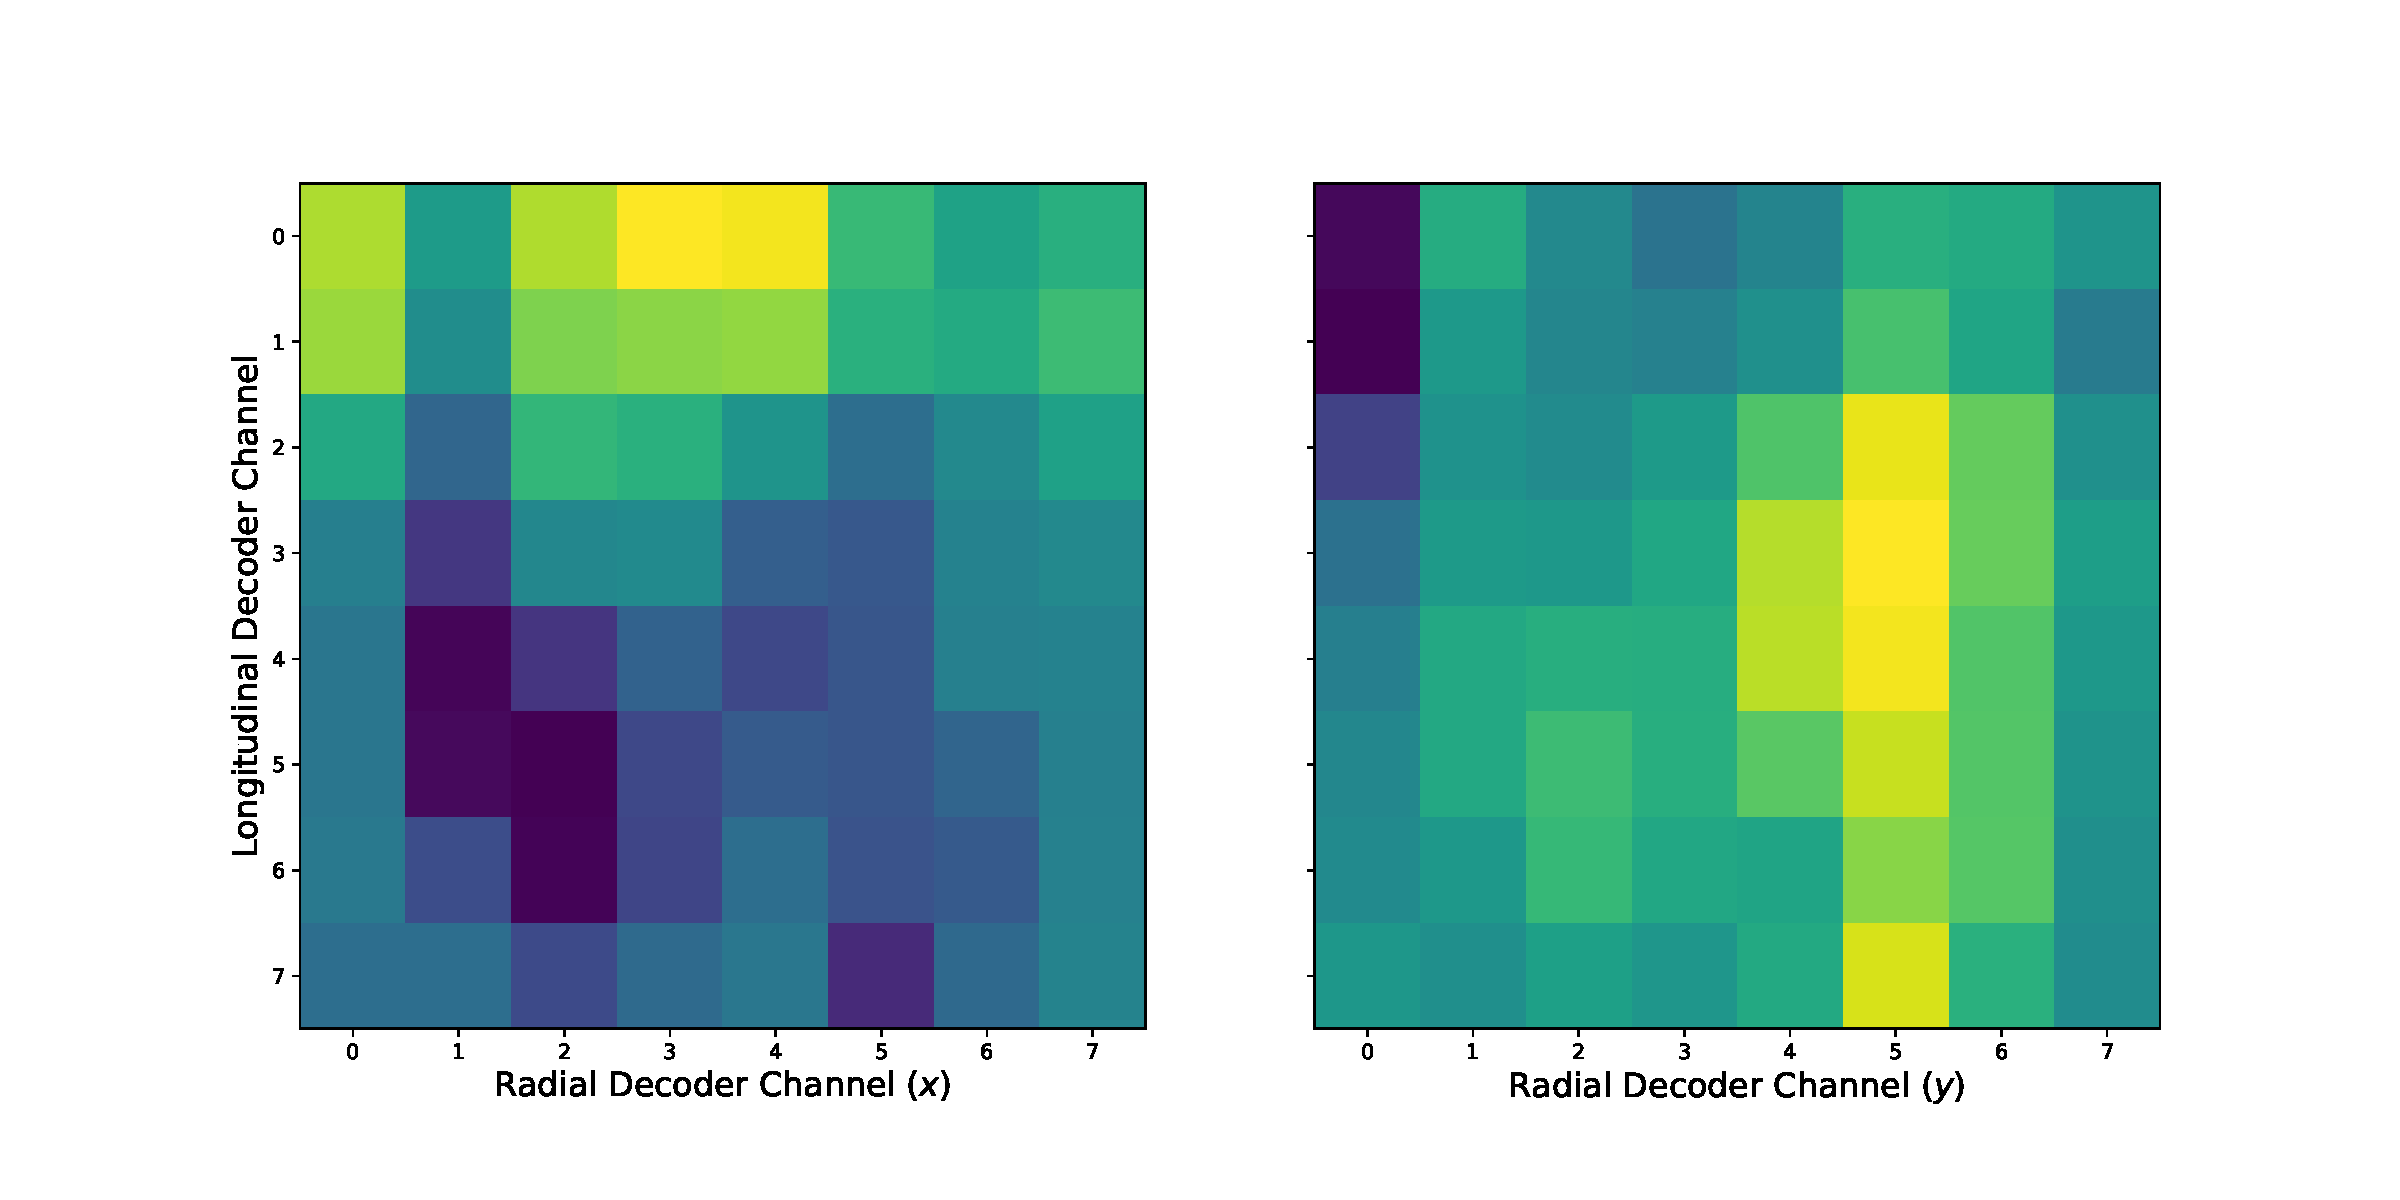
\includegraphics[width=1.0\textwidth]{methods/example_decoder.pdf}
  \caption[Example subject decoder]{Example EMG-to-force decoders from a single subject. The ``center hold, reach out'' task works by mapping 64 channels of EMG activity from subjects' forearms to a 2-dimensional force vector, a component acting in the $x$ and $y$ directions within the task's linear dynamics. Depicted here are the two 64-dimensional ``decoders'' arranged as the EMG electrodes were arranged on subjects' arms (along the arm, longitudinally, and around the arm, radially). The left plot shows the $x$ force decoder, and the right plot the $y$.}\label{fig:example_decoder}
\end{figure}



\subsection{Center Hold Reach Out}

``I would be most interested to hear how u are thinking of approaching the analysis. I.e. you have a bunch of channels, movements, tasks what is the workflow to get from that raw data into something manageable/useful?''

What does the basic data look like, discuss the shape of the data we have
46 Subjects x 12 targets x 45 trials x ~5k timepoints x 64 channels + 2 x 14 x Movements task + 2x Calibration task


\begin{figure}[tph]
  \centering
  \includegraphics[width=1.0\textwidth]{methods/filtering_steps.pdf}
  \caption[Data filtering steps]{Data from a single trial showing each step of preprocessing. The prototype preprocessing pipeline is highpass at 50Hz, rectification, and lowpass at 5Hz. The within-trial, per-channel means are subtracted from each trial. This matches what is typically done in the literature to find a correlate of intended force[@sangerBayesianFilteringMyoelectric2007;@churchlandNeuralPopulationDynamics2012a;@churchlandNeuralVariabilityPremotor2006;@sussillo2015]. There is significant room for improvement on this workflow, as discussed in the text.}\label{fig:filtering}
\end{figure}

\begin{figure}[tph]
  \centering
  \includegraphics[width=1.0\textwidth]{methods/example_trajectories.pdf}
  \caption{Point mass position trajectories in two-dimensional task space during the center-hold, reach-out task with 32 targets spaced evenly around the unit circle (shown with red borders). Color corresponds to target numbers, with target zero located at (0,1). Target order was randomized. Training was conducted over 3 blocks each with 32 trials, 1 trial per target.}\label{fig:example_trajectories}
\end{figure}

In this task, the 32-dimensional EMG electrode activity vector is mapped to a 2D force acting on a point mass shown on the screen. The mapping $M\in\mathbb{R}^{2 x 32}$ maps 8 ``columns'' each consisting of 4 electrodes placed in a line down the length of the forearm each to one of 2D root of unity. Each column of electrodes is thus mapped to one of 8 two-dimensional force vectors. In this experiment, the point mass has zero inertia and zero friction and as such displays a direct, though redundant, readout of the EMG signal. The task asks the subject to reach one of 32 equally spaced targets on each trial. Subjects must hold in the center of the task space for a designated period of time, after which the target appears. Subjects then have a time window reach the target. Data from one subject was recorded for three blocks in one session. Each block consisted of 32 trials, one per target in a randomized order.

A graphic showing the mappings from electrodes to force directions is shown in \Cref{fig:columns}. While there are 8 possible force vectors the subject can modulate by controlling the electrode activity on each of her 8 columns, the EMG mapping is ultimately a projection onto the 2D plane. Since the EMG signal is nonnegative, the subject could technically modulate just four modes of electrode activity, the minimum number needed to span the task space, to reach all 32 targets. This mapping was chosen in order to provide a simple starting point to explore the virtual EMG task. There are no added environmental dynamics, only a redundant readout of force, and the signal is processed online in the same manner as in the offline analyses. This task or a variant we think can serve as a foundation upon which we can build more complex mappings and virtual environments. Task space trajectories from each block are shown in \Cref{fig:trajectories}. The fraction of trials resulting in hold timeouts, reach timeouts, and target hits are shown over blocks in \Cref{fig:hit_fraction}.



\section{Data Validity}

Show that we can reproduce the data offline

Compare calibration to movement in terms of variance, rank, some metric of dispersion in EMG space.
How uniformly can subjects reach their EMG space? E.g. compared to a gaussian with the same statistics?
The calibration task defines the decoder, and thus it is worth confirming that it is successful in encouraging subjects to explore their EMG space. We can compare their activity to the natural movement datasets as a baseline.

Hypothesis: Variance in the calibration datasets is higher than in the natural movement dataset, even taking all natural movements together. This implies that the calibration dataset encourages exploration of a wider EMG space than that of natural movement.

We used NMF to produce decoders from one of the calibration task datasets. If we run NMF on the second calibration task dataset and compare the results to what was used in the task, are the results similar? This would confirm that the EMG space was adequately captured. We can define a distance metric between the two decoders and test if this correlates with performance. Differences in the decoders implies that our experimental decoder did not capture the EMG space adequately enough to provide a reasonable learning challenge.
Hypothesis: we will see similar results from the second NMF run, which will reject the hypothesis that our decoder does not well-represent subjects’ EMG movement space.
Hypothesis: inter-decoder distance within subjects will correlate negatively with performance (different decoders, less performant). This implies that the decoder’s capturing of whole EMG space, opposed to a subspace, enables subjects to perform better on the task. We expect a crossover point here– you want an EMG search space large enough to encompass the task itself, but small enough not to provide too great of a search task for subjects.

% \begin{figure}[tph]
%   \makebox[\linewidth][c]{%
%       \centering
%       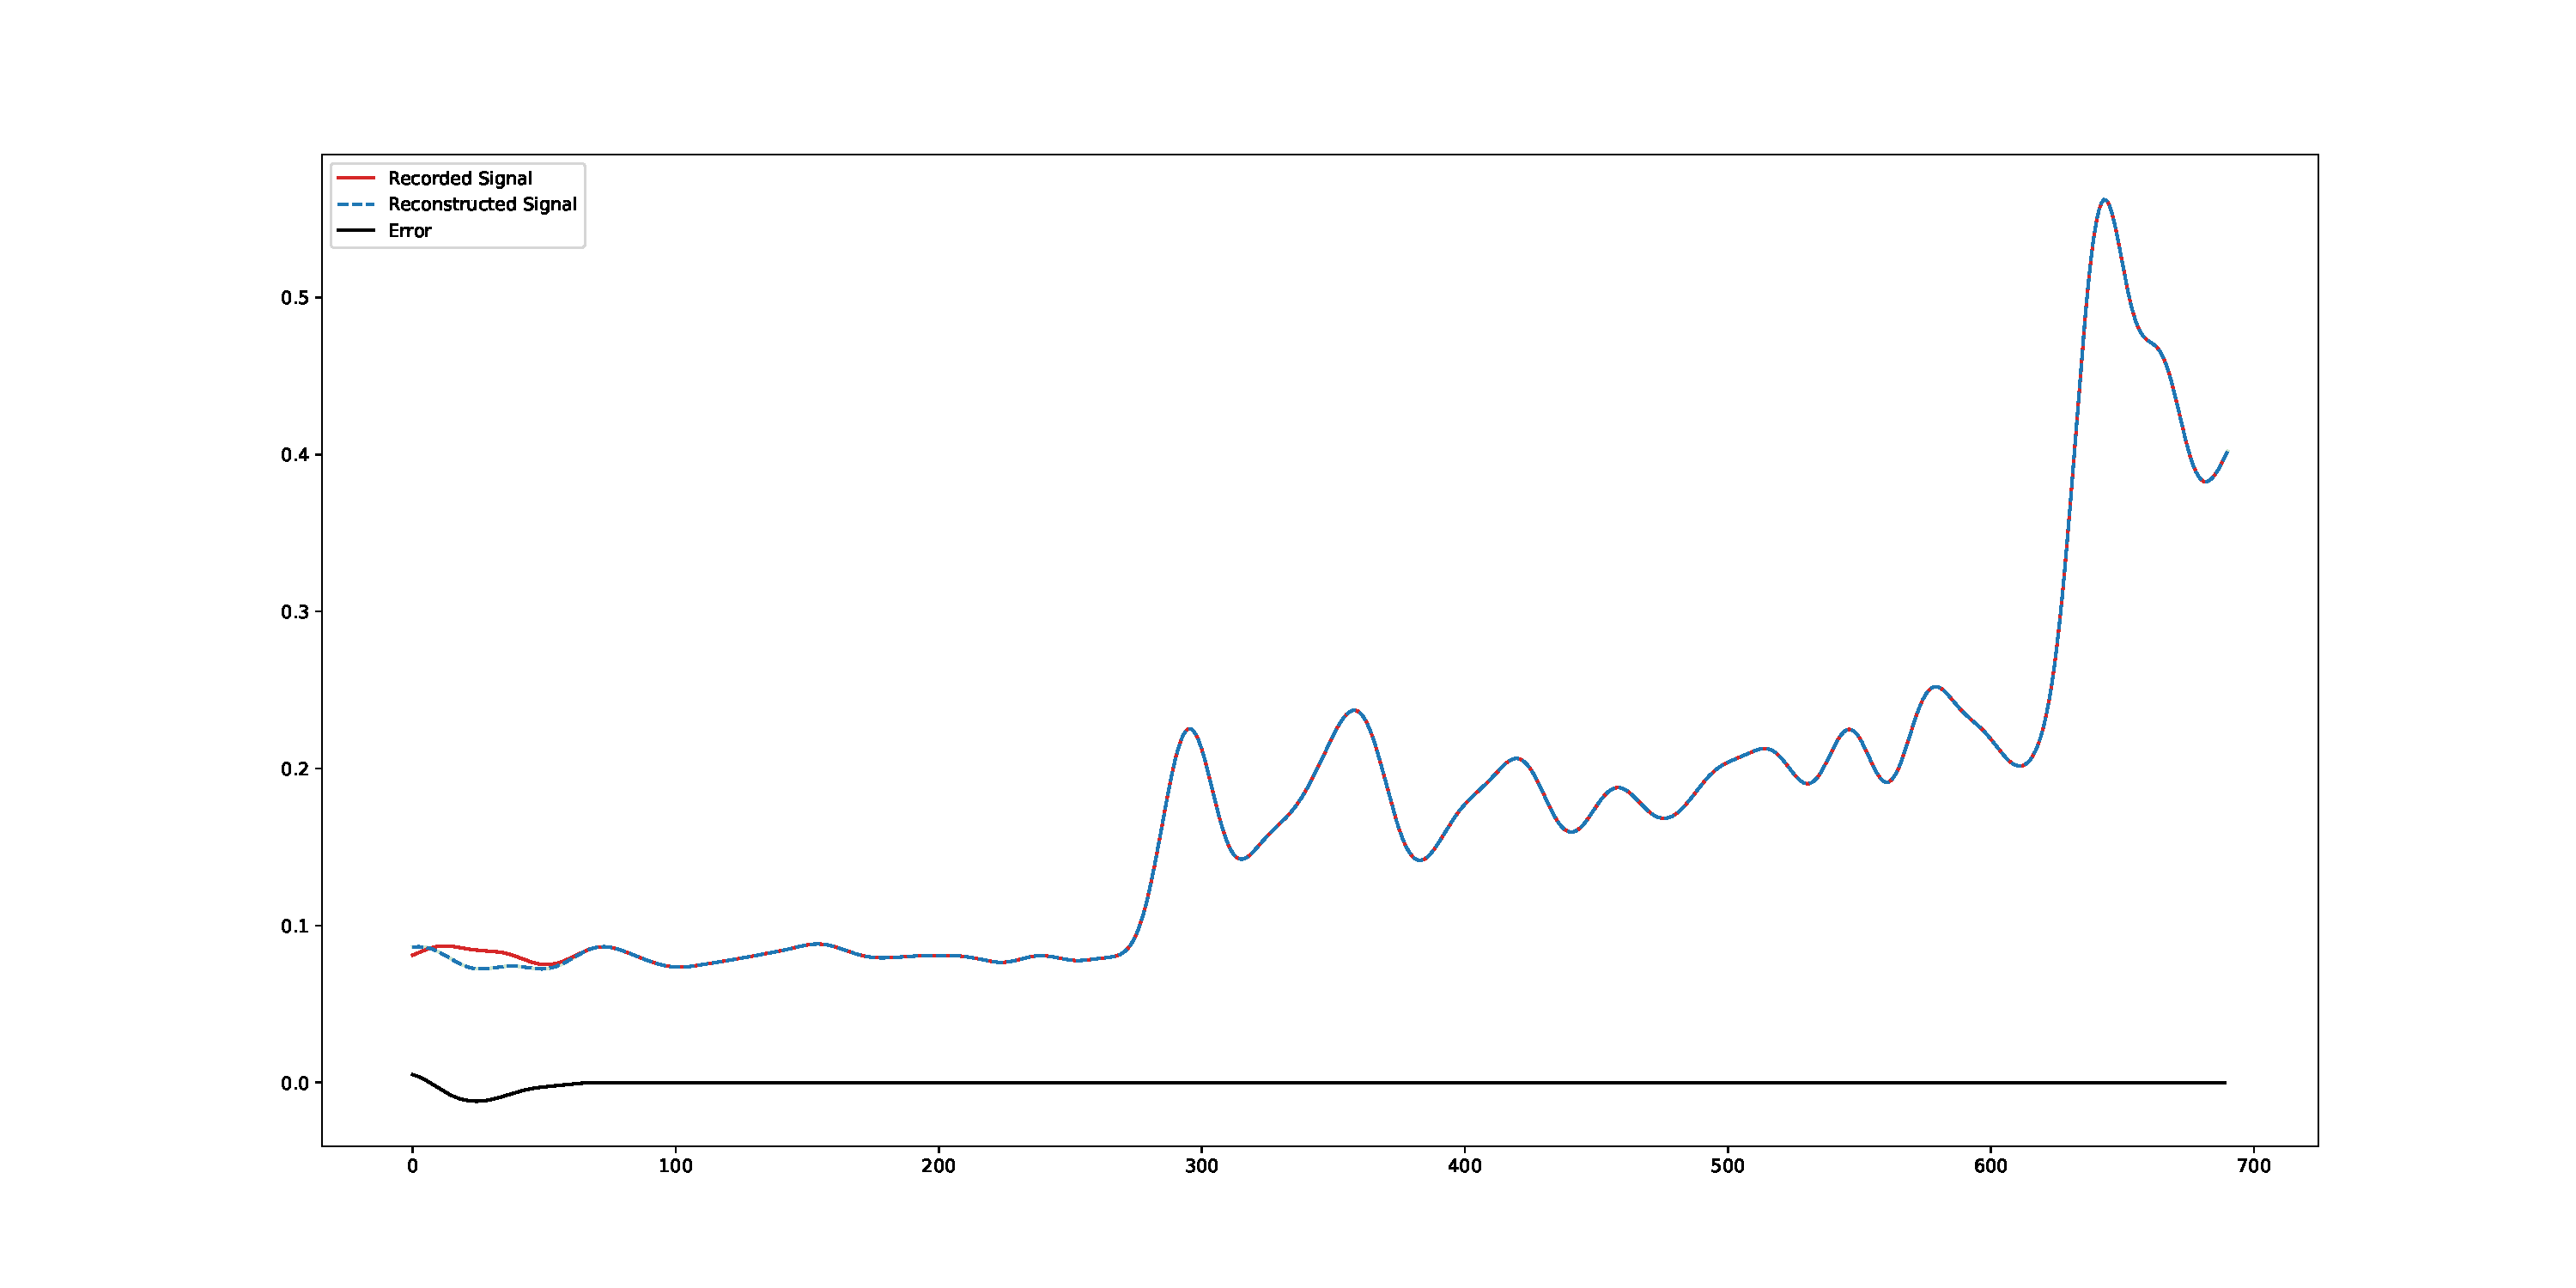
\includegraphics[width=1.3\textwidth]{analysis/reconstructed_emg.pdf}
%       }
%   \caption{Blah blah blah blah}\label{fig:behavior}
% \end{figure}

% \begin{figure}[tph]
%   \makebox[\linewidth][c]{%
%       \centering
%       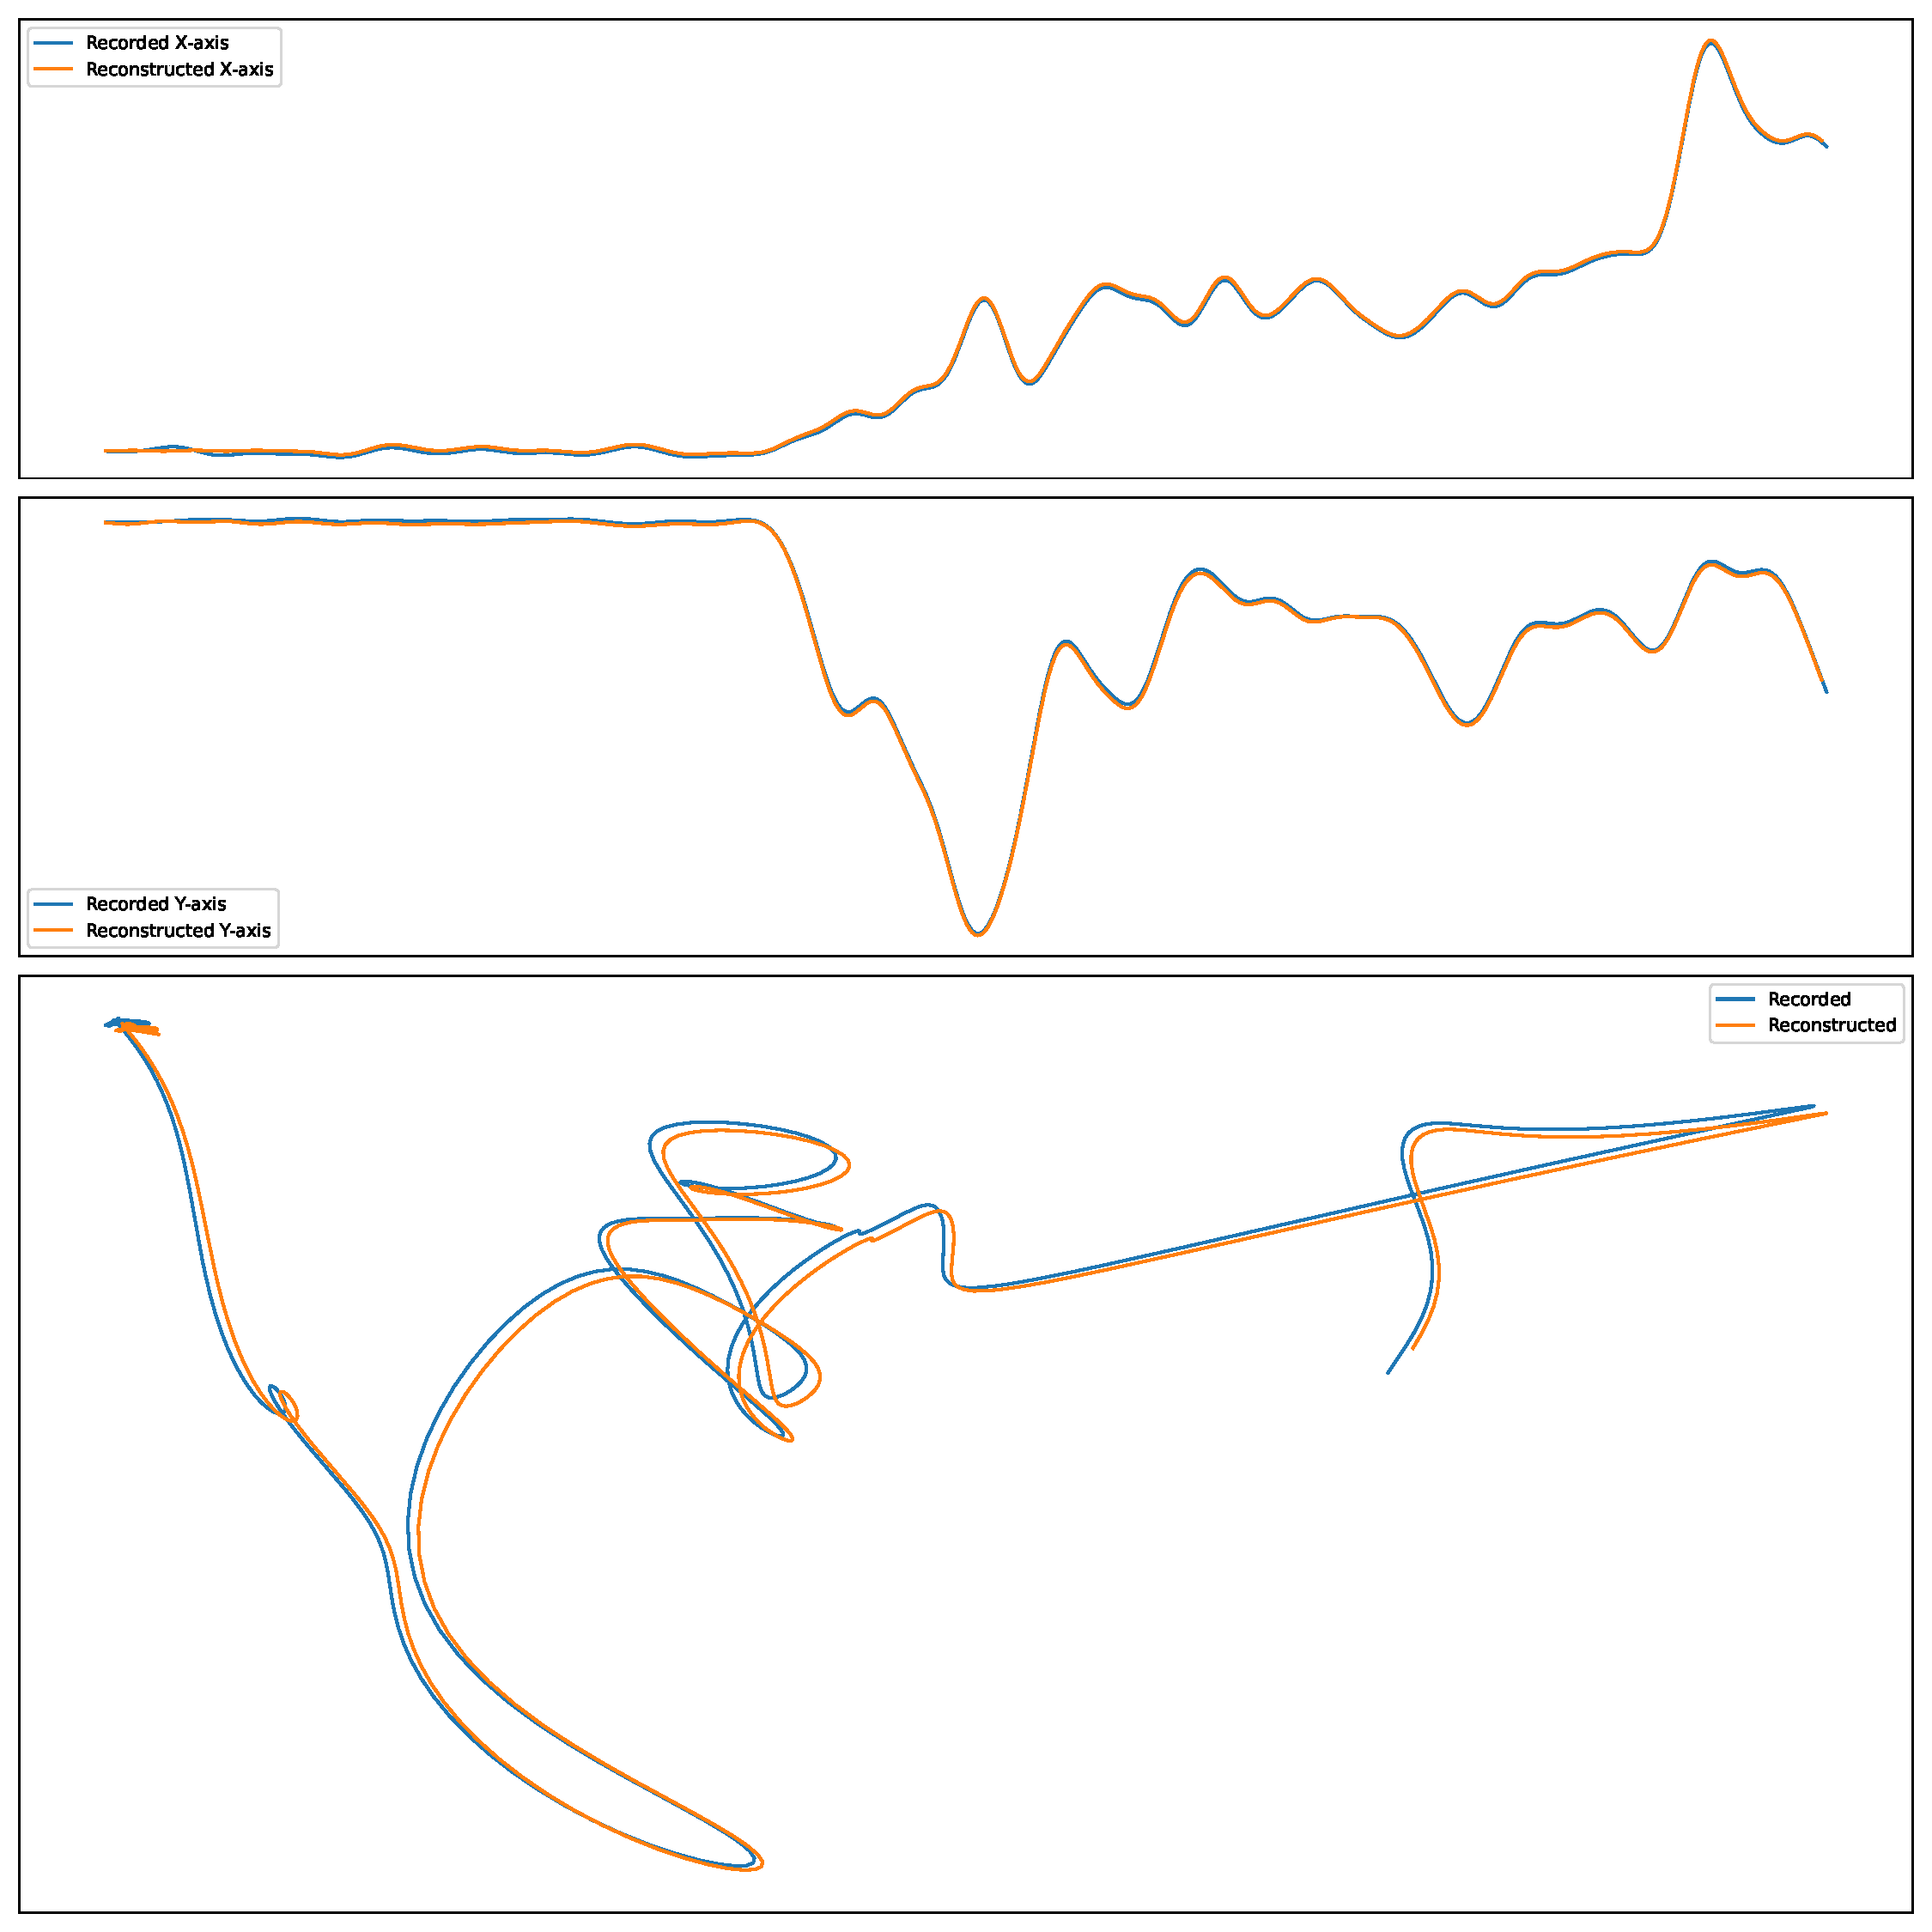
\includegraphics[width=1.3\textwidth]{analysis/reconstructed_trajectory.pdf}
%       }
%   \caption{Blah blah blah blah}\label{fig:behavior}
% \end{figure}



\section{Activity Filter}


Explain log filtering here?


Work back through the activity filter thing to make sure it makes sense statistically and we can defend it

Norm of EMG → histogram per trial → look at the distribution of this, should we log-transform it into a rough gaussian? → what is the variance cutoff we should use here? Mean +/ N*sigma, what is N to reject outliers? What do we do if the data isn’t gaussian even after log transforming?

Once we have our cutoff, we mask emg leaving only samples that fit within our defined activity window

Visualize norm histograms to check for outliers, weirdness

Explain the filtering process, both the data and the activity filtering. Talk about the log-normal transformation.

Remove offsets from EMG – show test
Capture “active” parts of EMG signal based on spatial norm – show test compared densities of movement before and after filtering?
Remove artifacts and outliers from EMG – Mahalanobis compared to active mean – show test
Use these “masks” on subsequent analyses

% for movement and calibration data
% log_norm = np.log(np.linalg.norm(signal,axis=1))
% mean_log_norm = np.mean(log_norm)
% std_log_norm = np.std(log_norm)
% # assuming large samples and rv being lognormal, this is roughly the 30th percentile
% mask = log_norm > (mean_log_norm - 0.5*std_log_norm)

% for trial data:
% log_norm = np.log(np.linalg.norm(signal,axis=1))
% mean_log_norm = np.mean(log_norm)
% std_log_norm = np.std(log_norm)
% # assuming large samples and rv being lognormal, this is roughly the 30th percentile
% mask = log_norm > (mean_log_norm - 0.0*std_log_norm)

% cutoffs for all data:
% samples = analysis.remove_nan_rows(subject_stack.transpose(0,1,3,2).reshape(-1,64))
% lognorms = np.log(np.linalg.norm(samples,axis=1))
% return (np.percentile(lognorms,1), np.percentile(lognorms,99.9))
% movement and calibration: 99.5
% trial: 99.9

\begin{figure}[tph]
  \begin{minipage}[b]{\linewidth}
    \centering
    \includegraphics[width=\textwidth]{methods/log_hist_movement.pdf}
    \subcaption{}
    \vspace{4ex}
  \end{minipage}\\
  \begin{minipage}[b]{\linewidth}
    \centering
    \includegraphics[width=\textwidth]{methods/log_hist_calibration.pdf}
    \subcaption{}
    \vspace{4ex}
  \end{minipage}\\
  \begin{minipage}[b]{\linewidth}
    \centering
    \includegraphics[width=\textwidth]{methods/log_hist_trial.pdf}
    \subcaption{}
    \vspace{4ex}
  \end{minipage}
  \caption[Log transforming EMG]{Activity filter!}\label{fig:log_hist}
\end{figure}

% \begin{figure}[tph]
%   \centering
%   \includegraphics[width=1.0\textwidth]{methods/activity_filter.pdf}
%   \caption[Activity filter example trial]{Activity filter!}\label{fig:activity_filter}
% \end{figure}

\begin{figure}[tph]
  \begin{minipage}[b]{0.7\linewidth}
    \centering
    \includegraphics[width=\textwidth]{methods/activity_filter_good_trial.pdf}
    \subcaption{}
    \vspace{4ex}
  \end{minipage}%%
  \begin{minipage}[b]{0.3\linewidth}
    \centering
    \includegraphics[width=\textwidth]{methods/trajectory_filter_good_trial.pdf}
    \subcaption{}
    \vspace{4ex}
  \end{minipage}
  \begin{minipage}[b]{0.7\linewidth}
    \centering
    \includegraphics[width=\textwidth]{methods/activity_filter_long_trial.pdf}
    \subcaption{}
    \vspace{4ex}
  \end{minipage}%%
  \begin{minipage}[b]{0.3\linewidth}
    \centering
    \includegraphics[width=\textwidth]{methods/trajectory_filter_long_trial.pdf}
    \subcaption{}
    \vspace{4ex}
  \end{minipage}
  \caption[Activity filter for EMG and trajectories]{Activity filter!}\label{fig:activity_filter}
\end{figure}


\cleardoublepage\printendnotes%
\ifSubfilesClassLoaded{%
    \newpage%
    \bibliography{../bib/bibliography}%
}{}%
\end{document}